%% LyX 2.0.0rc2 created this file.  For more info, see http://www.lyx.org/.
%% Do not edit unless you really know what you are doing.
\documentclass[english,multicols]{article}
\usepackage{amstext}
\usepackage{fontspec}
\usepackage{listings}
\usepackage{array}
\usepackage{varioref}
\usepackage{float}
\usepackage{textcomp}
\usepackage{multirow}
\usepackage{graphicx}
\usepackage[authoryear]{natbib}

\makeatletter

%%%%%%%%%%%%%%%%%%%%%%%%%%%%%% LyX specific LaTeX commands.
%% Because html converters don't know tabularnewline
\providecommand{\tabularnewline}{\\}
\floatstyle{ruled}
\newfloat{algorithm}{tbp}{loa}
\providecommand{\algorithmname}{Algorithm}
\floatname{algorithm}{\protect\algorithmname}

%%%%%%%%%%%%%%%%%%%%%%%%%%%%%% Textclass specific LaTeX commands.
\newfontfamily{\TH}[Scale=1.1]{Ayuthaya}
\newcommand{\thai}[1]{{\TH #1}}

%%%%%%%%%%%%%%%%%%%%%%%%%%%%%% User specified LaTeX commands.
\usepackage{IJCNLP2011}

\@ifundefined{showcaptionsetup}{}{%
 \PassOptionsToPackage{caption=false}{subfig}}
\usepackage{subfig}
\makeatother

\usepackage{xunicode}
\usepackage{polyglossia}
\setdefaultlanguage{english}
\begin{document}

\title{Automatic Transformation of the Thai Categorial Grammar Treebank
to Dependency Trees}


\author{~\\
~\\
~\\
~\\
}
\maketitle
\begin{abstract}
A method for deriving an approximately labeled dependency treebank
from the Thai Categorial Grammar Treebank has been implemented. The
method involves a lexical dictionary for assigning dependency directions
to the CG types associated with the grammatical entities in the CG
bank, falling back on a generic CG to CDG mapping in case of unknown
words. Currently, just a handful of the trees in the Thai CG bank
cannot unambiguously be transformed into directed dependency trees.
Derived dependency arcs are optionally labeled with a learned classfier,
achieving $\approx75\%$ label accuracy on a sample set. In the process,
a number of annotation errors in the CG bank were identified and corrected.
Although rather limited in its coverage, excluding e.g. long-distance
dependencies, topicalisations and longer sentences, the resulting
treebank is believed to be sound in terms structural annotational
consistence and a valuable complement to the scarce Thai language
resources in existence.
\end{abstract}

\section{Introduction}

Syntactic resources play an essential role for the majority of NLP
applications, but for Thai language, openly available syntactic resources
are few in number: So far, the only reported resources are the CG
treebank \citep{ruangrajitpakorn2009asyntactic} and the NAiST dependency
bank \citep{wacharamanotham2007thedevelopment,sudprasert2008dependency}
--- others being either unpublished or minuscule in size. These treebanks
were approved manually by linguists, and therefore expectedly reliable
in terms of accuracy. However, each resource is fairly limited in
size. Rather than relying exclusively on labor-intensive manual annotation
for further expanding the resources, it would be economically sound
to leverage existing efforts and transform an existing treebank in
one grammar into the another.


\subsection{Categorial grammar}

Categorial grammar (CG) is a lexicalised theory in natural language
syntax motivated by the principle of constitutionality and organised
according to the syntactic elements \citep{ajdukiewicz1935diesyntaktische,steedman2000thesyntactic},
and forms the theoretical basis for the Thai CG treebank. The resource
building effort has been very fruitful, but there remains phenomena
of Thai languge, including long-range dependencies and topicalisation
\citep{warotamasikkhadit1997fronting}, which are unhandled by the
instantiation of CG currently in use. 

Additionally, although Thai language belongs to a fixed word order
typology, Thai spoken language exhibits some flexibility in word order,
due to the occasional preference of Thai language users for correspondance
in rhyme. As an example, consider the following sentence%
\footnote{The Thai adverbialising prefix \thai{อย่าง} can be likened
to the English {}``-ly'' suffix, which produces an adverbial form
from an adjective. Artificial word boundaries has beeen inserted for
clarity.%
}:\\


\begin{minipage}[t]{0.9\columnwidth}%
\begin{flushleft}
\thai{อังกฤษ คิดค้น อย่าง หนัก วัคซีนป้องกันเชื้อไวรัสไข้หวัดนก}
\par\end{flushleft}

(\textbf{Lit}: England/NE invent/V {}``-ly''/ADVPFX heavy/ADJ avian\_flu\_vaccine/NP)

\begin{flushleft}
{}``The British are strenuously developing an Avian Flu vaccine.''
\\
~\\

\par\end{flushleft}%
\end{minipage}

The adverbial compound formed by \thai{อย่าง หนัก}
({}``strenuously'') conventionally occurs after the direct object,
but is in this sentence, it is realised in the pre-direct object position%
\footnote{When language users exploit this flexibility in word order to produce
aesthetically pleasing sound patterns, it results in a marked form,
but the phenomenon is nonetheless productive, and encountered frequently
enough to necessitate handling in NLP applications. %
} in order for the last syllable of \thai{อย่าง หนัก}
to rhyme with the first syllable of \thai{วัคซีน} ({}``vaccine'').
To some degree, this phenomenon from spoken language shines through
in written language, especially in the domains of news and recent
politics, and is causing a challenge for the employment of CG grammar. 

\begin{figure*}
\begin{centering}
\includegraphics{dep_repr_ambiguity}
\par\end{centering}

\caption{Examplar of ambiguity arising only in dependency representation \citep{daum2004automatic}\label{fig:Examplar-of-ambiguity}}
\end{figure*}



\subsection{Dependency representation}

In recent years, dependency representation has seen a dramatic increase
in interest, likely due to a number of appealing properties of the
representation. In comparison to phrase structure grammar, dependency
structures provide a relatively direct encoding of predicate-argument
structure, which is relevant to subsequent analyses \citep{nivre2005dependency}.
Dependency representation is arguably better suited for languages
with flexible word order. Additionally, having no non-terminal nodes,
dependency structures are often perceived as leaving room for less
ambiguity as well as being more computationally managable.

Certainly, dependency representation has drawbacks of its own in terms
of ambiguity, some of which are specific to dependency representation.
In particular, Figure \ref{fig:Examplar-of-ambiguity} shows a construction
with an unambiguous constituent structure, which in dependency space
is ambiguous with respect to the attachment of the adverb \citep{daum2004automatic}. 

Furthermore, dependency structure allows for a number of ways to represent
coordinated phrases, some having the \emph{coordinating conjunction
as head} (CCH) of the coordinate structure, and a special dependency
label \emph{CJT} that does not describe the grammatical function of
the conjuncts (Figure \ref{fig:CCH}). Another option is having the
\emph{coordinating conjunction as dependent} (CCD) of one of the conjuncts,
thus allowing one conjunct to occur with a dependency label expliciting
its grammatical function (Figure \ref{fig:CCD}). \citet{mcdonald2007characterizing}
offer a thorough review of these and other candidate analyses in use.
Unfortunately, none of the conceivable representations are unproblematic
from a linguistic perspective \citep{daum2004automatic}, or offer
the same transparency as the coordination rules of CCG do \citep{boonkwan2009amemorybased}.

\begin{figure}
\begin{centering}
\subfloat[CCH\label{fig:CCH}]{\begin{centering}
\includegraphics[width=0.75\columnwidth]{cch}
\par\end{centering}

}
\par\end{centering}

\begin{centering}
\subfloat[CCD\label{fig:CCD}]{\begin{centering}
\includegraphics[width=0.75\columnwidth]{ccd}
\par\end{centering}

}
\par\end{centering}

\centering{}\caption{Two possible analyses of a coordination \citep{kubler2009dependency}\label{fig:coord}}
\end{figure}


Nonetheless, given the availability of generally applicable, trainable
dependency parsers, and reports of beneficial applications of dependency
analysis in tasks such as word-alignmeent \citep{ma2008improving}
and reordering \citep{chang2009discriminative} for statistical machine
translation, a dependency treebank of good quality is a highly desirable
resource.


\subsection{Outline}

The rest of the paper is organised as follows. In Section \ref{sec:Related-work}
we briefly review other works dealing with similar transformations,
before presenting the approach taken in this work in Section \ref{sec:Methodology}.
Section \ref{sec:Experiments} describes the experimental setting
and results, which are discussed in Section \ref{sec:Discussion}.
Finally, Section \ref{sec:Conclusion} concludes the paper. 


\section{Related work\label{sec:Related-work}}

In preperation for the CoNLL-X shared task on dependency parsing \citep{buchholz2006conllxshared},
a number dependency trees were derived from a number of constituency-based
phrase structure treebanks, most of which has grammatical function
(e.g. {}``subject'' and {}``object'') as part of the annotation.
The conversion process for such treebanks would involve a \emph{head
table} with rules of the form 
\begin{itemize}
\item {}``the head child of a VP/clause is the child with the HD/predicator/hd/Head
function'' and 
\item {}``{[}the dependency label{]} for a token is the function of the
biggest constituent of which this token is the lexical head''. 
\end{itemize}
The case of the Thai CG bank is different, as it does not directly
contain any grammatical functions. On the other hand, identifying
head tokens is relatively straight-forward when augmenting the CG
annotation with dependency directions \citep{ruangrajitpakorn2010acurrent}. 

\citet{chanev2006dependency} faced a similar situation in their transformation
of the BulTreeBank to dependency representation. Heads were first
identified from explicitly stated rules in a head table. Lacking explicit
grammatical functions in the source treebank, they explored a heuristic
rule-based approach for the labeling with a \emph{dependency table,}
containing rules based on parent constituents. Although good results
are achieved, they report of errors like mistaken subjects and objects. 


\section{Methodology\label{sec:Methodology}}

The situation with the Thai CG bank is a little different. Together
with a set of combinatory grammer rules, the CG type tags and bracketing
present in the treebank unambigously specify the constituent structure
of the treebank sentences. When the CG type tags are augmented with
dependency directions, a dependency tree can be derived with relative
ease from the CG-based constituents. Grammatical functions, however,
are not immediately evident from the CG trees. 

We first describe a relatively straight-forward method for deriving
the dependency trees, and next consider the more daunting task of
assigning functional labels to the dependency arcs. Figure \ref{fig:Transformation-overview}
shows a schematical overview of the proprosed method.

\begin{figure*}
\begin{centering}
\includegraphics[width=1\textwidth]{process}
\par\end{centering}

\centering{}\caption{Transformation overview\label{fig:Transformation-overview}}
\end{figure*}



\subsection{Terminology}

For any given CG type $t$, we use thethe \emph{arity} (admittedly
a bit sloppily) to denote the ordered list of arguments expected by
a type. The arity of the type $\mathtt{s\backslash np/ws/np}$ is
thus $\mathtt{/np}$, $\mathtt{/ws}$ and $\mathtt{\backslash np}$
--- that is, 
\begin{itemize}
\item a noun phrase from the right, followed by 
\item a subordinate clause beginning with the Thai word \thai{ว่า}
({}``that'', subordinate clause marker), and 
\item another noun phrase from the left.
\end{itemize}
Complementary, we define the \emph{yield} of $t$ as the set of possible
CG types which may result from functional application of a CG rule.
The transitive verb type $\mathtt{s\backslash np/np}$, for example,
yields
\begin{itemize}
\item $\mathtt{s\backslash np}$ and 
\item $\mathtt{s}$
\end{itemize}
after receiving a $\mathtt{np}$ to the right, and another $\mathtt{np}$
to the left, respectively. This is simply the basic combinatory CCG
rules:

\begin{eqnarray*}
\textrm{X/Y}\;\;\;\textrm{Y} & \Rightarrow & \textrm{X}\\
\textrm{Y}\;\;\;\textrm{X\textbackslash Y} & \Rightarrow & \textrm{X}
\end{eqnarray*}



\subsection{Dependency directions}

The first transformation step, which can rightly be regarded as a
necessary preprocessing step before the actual transformation, involves
a lexical dictionary for assigning dependency directions to the CG
types associated with the grammatical entities in the CG bank, falling
back on a generic CG to CDG mapping in case of unknown words. 

Note that only terminal nodes will have assigned dependency directions
assigned by this procedure. Dependency directions are propagated to
non-terminal nodes in a bottom-up fashion by the procedure $\mathtt{propagateDirections}$
(Algorithm \ref{alg:propagating}). In identifying which child to
adopt dependency directions from, the parent node type is checked
against the yield\emph{ }of each child node. 

\begin{algorithm}
\begin{lstlisting}[basicstyle={\footnotesize},language=Python]
def propagateDirections(node):
  for child in node.children:
    propagateDirections(child)
  if node.hasDependencyDirection:
    return
  for child in node.children:
    if child.yields(node.type):
      node.depDirs = child.depDirs
      break
\end{lstlisting}


\caption{Pseudo-code for propagating dependency directions to non-terminal
nodes.\label{alg:propagating}}
\end{algorithm}



\subsection{Head finding}

Dependency arcs are assigned by a procedure that implements the CDG
dependency derivation rules introduced by \citet{ruangrajitpakorn2010acurrent}
(motivated by \citealp{collins1999headdriven}). Let $c:d$ signify
a CDG type $c$ and a dependency structure $d$, and the notion $h(\mathrm{d}_{1})\rightarrow h(\mathrm{d}_{2})$
represent a dependency arc between the head of $d_{1}$ and the head
of $d_{2}$ (with $h(\mathrm{d}_{1})$ governing $h(\mathrm{d}_{2})$)
. Then the derivation rules are:

\begin{eqnarray*}
\textrm{X/<Y:d}_{1}\;\;\textrm{Y:d}_{2} & \Rightarrow & h(\mathrm{d}_{1})\leftarrow h(\mathrm{d}_{2})\\
\textrm{X/>Y:d}_{1}\;\;\textrm{Y:d}_{2} & \Rightarrow & h(\mathrm{d}_{1})\rightarrow h(\mathrm{d}_{2})\\
\textrm{Y:d}_{1}\;\;\textrm{X\textbackslash<Y:d}_{2} & \Rightarrow & h(\mathrm{d}_{1})\leftarrow h(\mathrm{d}_{2})\\
\textrm{Y:d}_{1}\;\;\textrm{X\textbackslash>Y:d}_{2} & \Rightarrow & h(\mathrm{d}_{1})\rightarrow h(\mathrm{d}_{2})
\end{eqnarray*}


In addition to the standard combinatory rules for forward and backward
functional application above, the Thai CG bank makes use of a CCG-style
\emph{serialisation} rule to handle e.g. serial verb constructions,
which are used in Thai (and Chinese) to express serial or consecutive
events. As \citet{boonkwan2009amemorybased}, we take the notion of
a \emph{serial verb construction} to mean a series of verbs or verb
phrases without explicit connectives marked with (or understood to
have) the same grammatical categories, and sharing at least one common
argument, typically a subject. 

As an example, the verbs \thai{ตรวจ} ({}``examine'') and
\thai{พบ} ({}``find'') occur serially in the following sentence%
\footnote{Articifial word boundaries inserted for clarity.%
} from the CG bank, indicating a resultative course of events \citep{thepkanjana2009resultative}:\\


\begin{minipage}[t]{0.9\columnwidth}%
\begin{flushleft}
\thai{นักวิชาการ ตรวจ พบ ไวรัส โคโรน่า ใน ชะมด}
\par\end{flushleft}

\begin{flushleft}
(\textbf{Lit}: scientist/N examine/V find/V virus/N corona/N in/PP
otter-civet/N)
\par\end{flushleft}

\begin{flushleft}
{}``The scientist examined the otter-civet and found coronavirus.''
\par\end{flushleft}

\begin{flushleft}
~\\

\par\end{flushleft}%
\end{minipage}

We introduce a generalised derivation rule for serial constructions
which simply designates the head of the first dependency structure
as governing the head of the following dependency structure:

\begin{eqnarray*}
\textrm{X:d}_{1}\;\;\textrm{X:d}_{2} & \Rightarrow & h(\mathrm{d}_{1})\rightarrow h(\mathrm{d}_{2})
\end{eqnarray*}


The rule is generalised in the sense that it handles \emph{serial
noun constructions} as well as serial verb constructions. 

Further CCG-style combinatory rules, such as functional composition
and type raising, are not currently in use in the Thai CG bank, and
therefore not handled by the transformation. 

An outline of the head finding procedure is given as Algorithm \ref{alg:head-finding}.
Intuitively, the algorithm proceeds by, for each node in turn, beginning
at the terminal nodes, identifying sibling nodes which satisfy the
arity of the of the node CG type. For each sibling node satisfying
an argument, the dependency derivation rule is applied and the sibling
is removed. 

It is worth noting that while both terminal and non-terminal nodes
are involved in this process, we are only interested in assigning
dependency arcs to terminal nodes, as non-terminals are absent in
the all-terminal dependency structure. This is ensured by an implementation
detail of the procedure $\mathtt{registerHead}$ (omitted from Algorithm
\ref{alg:head-finding}), in which non-terminal nodes act as proxies
for their terminal heads.

\begin{algorithm}
\begin{lstlisting}[basicstyle={\footnotesize},language=Python]
def assignHeads(node):
  for c in node.nonterminalChildren:
    assignHeads(c)
  for c in node.terminalChildren:
    assignHeads(c)
  for arg in node.type.arguments:
    if arg.side == 'right':
      sibl = node.rightSiblings.first
    else
      sibl = node.leftSiblings.last
    break unless arg.matches(sibl)
    if arg.side == 'right':
      if arg.dependencyDir == '>':
        registerHead(sibl, node)
      else: # <
        registerHead(node, sibl)
      node.rightSiblings.shift
    else: # left
      if arg.dependencyDir == '>':
        registerHead(node, sibl)
      else: # <
        registerHead(sibl, node)
      node.leftSiblings.pop  
\end{lstlisting}


\caption{Pseudo-code for the head-finding procedure.\label{alg:head-finding}}


\end{algorithm}



\subsection{Dependency labeling\label{sub:Dependency-labeling}}

Although the CDG-augmentation of the CG treebank implies a dependency
structure for each sentence, there are no immediate clues available
about the specific grammatical functions of dependency arcs. Obviously,
there are some clear-cut cases: When a token with CDG type $\mathtt{((s\backslash<np)\backslash>(s\backslash<np))\backslash<num}$
modifies a token with CDG type $\mathtt{num}$, it must be an application
of a \emph{quantifier} (with dependency type {}``quan''), as exemplified
in Figure \ref{fig:Given-the-CDG}.

\begin{figure*}
\begin{centering}
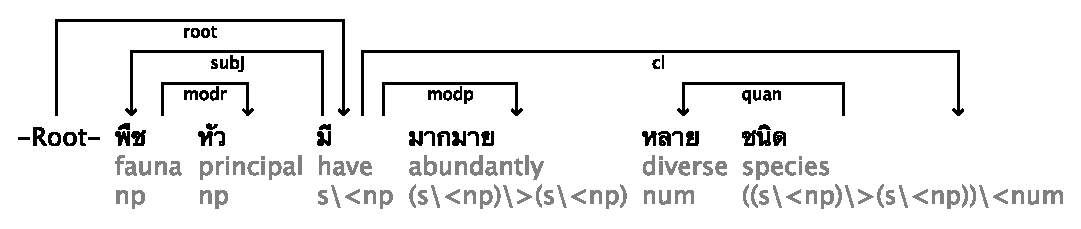
\includegraphics[width=0.75\textwidth]{deprels/quan}
\par\end{centering}

\caption{An unmistakekable labeling case: Given the CDG types of \protect\thai{หลาย}
({}``diverse'') and \protect\thai{ชนิด} ({}``species''),
the only dependency label supported by the examined data is {}``quan''
(\emph{quantifier}). \label{fig:Given-the-CDG}}
\end{figure*}


Other cases are less obvious. Even when taking dependency direction
and argument position into consideration, there are still cases with
several possible dependency types, as shown in Figure \ref{fig:Different-labeling}.

While for many practical purposes an unlabeled dependency structure
is sufficient, having proper dependency labels is nonetheless desirable.
In lack of an exact transformation, the approach explored in this
work relies instead on training a classifier to predict the correct
dependency label given local features of the tokens involved, as they
occur in the dependency structure derived from the CDG tree. Two feature
sets are suggested: The basic set comprising head and dependent CDG
type, as well as dependency direction ({}``L'' or {}``R'', as
seen from the dependent). The other set extends the basic set by including
surface forms.

\begin{figure}
\subfloat[Subject (subj)]{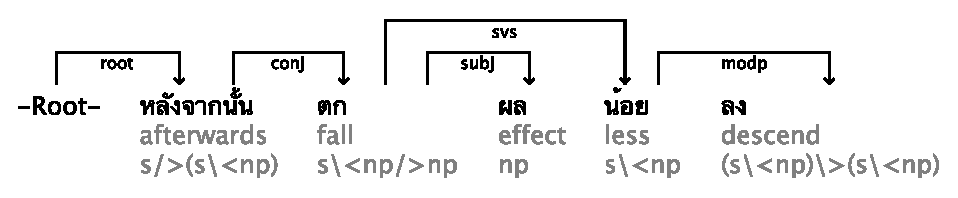
\includegraphics[width=1\columnwidth]{deprels/subj}

}

\subfloat[Direct object (dobj)]{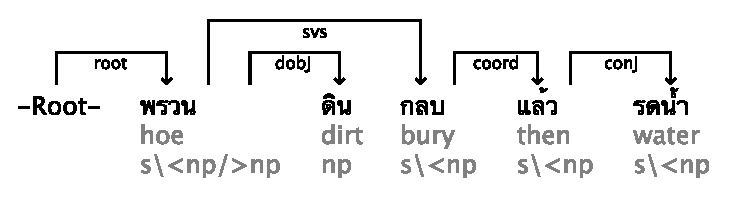
\includegraphics[width=1\columnwidth]{deprels/dobj}

}

\subfloat[adverbialiser (advm)]{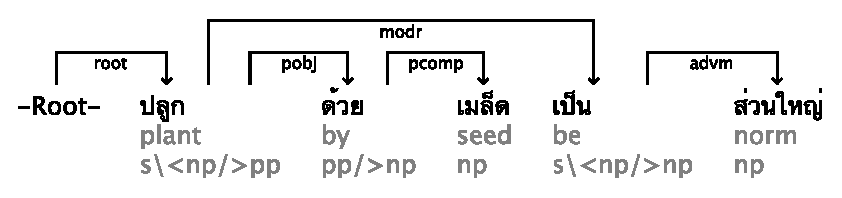
\includegraphics[width=1\columnwidth]{deprels/advm}

}\caption{Different labeling of left-pointing dependency arcs with $\mathtt{s\backslash<np/>np}$
as head CDG type and $\mathtt{np}$ as dependent CDG type. See Figure
\ref{fig:dep-types} for depency type abbreviations.\label{fig:Different-labeling}}
\end{figure}



\section{Experiments\label{sec:Experiments}}

The Thai CG bank made available for this research contains 1,428 CG
trees, comprised of
\begin{itemize}
\item 539 verb phrases or subject-omitted phrases ($\mathtt{s\backslash np}$),
\item 363 sentences ($\mathtt{s}$),
\item 372 noun phrases ($\mathtt{np}$) and
\item 4 prepositional phrases%
\footnote{As there is no explicit sentence boundary marker in Thai \citep{satayamas2004widecoverage},
it is often unclear what constitutes {}``a sentence''. The distribution
of tree types reflect the partitioning of token sequences made by
the treebank annotators for the purpose of treebanking.%
} ($\mathtt{pp}$).
\end{itemize}
The lexical dictionary used contains possible CDG types for 38.250
word forms, with an average of 2 types listed per word form. For six
of the word forms, the dictionary lists several possible dependency
directions for a single CG type. These confusable CDG types and the
dictionary entries they occur for are listed in Table \ref{tab:ambi-dict}.

\begin{table*}
\begin{tabular}{|l|c|c|l|}
\hline 
Word form(s) & CG type & Possible CDG equivalents & Interpretation\tabularnewline
\hline 
\hline 
\multirow{2}{*}{\thai{น่า}} & \multirow{2}{*}{$\mathtt{(s\backslash np)/(s\backslash np)}$} & $\mathtt{(s\backslash<np)/>(s\backslash<np)}$ & Adverb {}``please''\tabularnewline
 &  & $\mathtt{(s\backslash<np)/<(s\backslash<np)}$ & Auxiallary verb {}``should''\tabularnewline
\hline 
\thai{ตอนนั้น} ({}``at that time'') &  & \multirow{2}{*}{$\mathtt{s/>s}$} & \multirow{2}{*}{Conjunction}\tabularnewline
\thai{ตอนนี้} ({}``at present'') & \multirow{2}{*}{$\mathtt{s/s}$} &  & \tabularnewline
\thai{ขณะนั้น} ({}``at that moment'') &  & \multirow{2}{*}{$\mathtt{s/<s}$} & \multirow{2}{*}{Adverb of time}\tabularnewline
\thai{ขณะนี้} ({}``this moment'') &  &  & \tabularnewline
\hline 
\multirow{2}{*}{\thai{กับ}} & \multirow{2}{*}{$\mathtt{np\backslash<np/>np}$} & $\mathtt{np\backslash>np/>np}$ & Preposition {}``with''\tabularnewline
 &  & $\mathtt{np\backslash<np/>np}$ & Conjunction {}``and''\tabularnewline
\hline 
\end{tabular}

\caption{Entries in the lexical dictionary which are ambiguous with respect
to dependency direction\label{tab:ambi-dict}}
\end{table*}


An example sentence from the treebank affected by the ambiguous mapping
of the adverb \thai{ตอนนี้} ({}``at present'') is %
\footnote{The Thai auxillary verb \thai{กำลัง} indicates the present
participle, meaning \textquotedbl{}in the act of\textquotedbl{}, similar
to the English suffix, \textquotedbl{}-ing\textquotedbl{}. Articifial
word boundaries has been inserted for clarity.%
}:\\


\begin{minipage}[t]{0.9\columnwidth}%
\thai{ตอนนี้ เธอ กำลัง ยุ่ง มาก}

\begin{flushleft}
(\textbf{Lit}: this-moment/ADV she/PRON {}``-ing''/AUX busy/ADJ
very/ADV)
\par\end{flushleft}

\begin{flushleft}
{}``At this moment she is being very busy.''
\par\end{flushleft}

\begin{flushleft}
~\\

\par\end{flushleft}%
\end{minipage}

Examples of the latter two ambiguity classes of the lexical dictionary
(Table \ref{tab:ambi-dict}) were not encountered in the treebank
--- i.e. the affected word forms do not occur with an ambiguous CG
type. In dealing with these ambiguous entries in the lexical dictionary,
we simply (and naively) choose the first mapping option.

The generic CG to CDG mapping, used in addition to the lexical dictionary
as fallback for word forms not found in the lexical dictionary, also
exhibits some degree of ambiguity. The seven CG types with multiple
possible CDG equivalents are listed in Table \ref{tab:map}.

\begin{table}
\begin{centering}
\begin{tabular}{|c|>{\centering}p{4cm}|}
\hline 
CG type & Possible CDG equivalents\tabularnewline
\hline 
\hline 
$\mathtt{np\backslash np/np}$ & $\mathtt{np\backslash>np/>np}$\linebreak $\mathtt{np\backslash<np/>np}$\tabularnewline
\hline 
$\mathtt{s/s}$ & $\mathtt{s/>s}$\linebreak $\mathtt{s/<s}$\tabularnewline
\hline 
$\mathtt{s\backslash s}$ & $\mathtt{s\backslash>s}$\linebreak $\mathtt{s\backslash<s}$\tabularnewline
\hline 
$\mathtt{(s\backslash np)/(s\backslash np)}$ & $\mathtt{(s\backslash<np)/>(s\backslash<np)}$\linebreak $\mathtt{(s\backslash<np)/<(s\backslash<np)}$\tabularnewline
\hline 
$\mathtt{s/(s\backslash np)}$ & $\mathtt{s/>(s\backslash<np)}$\linebreak $\mathtt{s/<(s\backslash<np)}$\tabularnewline
\hline 
$\mathtt{s\ensuremath{\backslash(s\backslash np)}}$ & $\mathtt{s\backslash<(s\backslash<np)}$\linebreak $\mathtt{s\backslash>(s\backslash<np)}$\tabularnewline
\hline 
$\mathtt{s/(s\backslash np)/np}$ & $\mathtt{s/>(s\backslash np)/>np}$\linebreak $\mathtt{s/<(s\backslash np)/>np}$\tabularnewline
\hline 
\end{tabular}
\par\end{centering}

\caption{Cases of CD to CDG mappings which are ambigous with respect to dependency
direction\label{tab:map}}
\end{table}



\subsection{Dependency labeling }

To evaluate the classification-based approach to assigning dependency
labels, a sample of 678 labeled dependency edges from the NAiST dependency
treebank \citep{wacharamanotham2007thedevelopment} was used, along
with corresponding CDG trees obtained from a related work (manuscript
in preparation). The \emph{basic} and \emph{extended} feature sets
desribed in section \vref{sub:Dependency-labeling} were evaluated
with four different classifiers%
\footnote{Experiments with the learners were done using leave-one-out cross-validation,
with the exception of LibSVM, which was run using the standard K-fold
cross-validation of the easy.py script \citep{chang2001libsvma}.%
} (see Table \ref{tab:accuracy}).

\begin{table}
\centering{}%
\begin{tabular}{|l|r@{\extracolsep{0pt}.}l|r@{\extracolsep{0pt}.}l|}
\hline 
Classifier & \multicolumn{2}{c|}{Basic feats} & \multicolumn{2}{c|}{+forms}\tabularnewline
\hline 
\hline 
RandomForest-Weka & \multicolumn{2}{c|}{61.8\%} & \multicolumn{2}{c|}{69.5\%}\tabularnewline
\hline 
LibSVM & \multicolumn{2}{c|}{\textbf{62.8\%}} & \multicolumn{2}{c|}{\textbf{74.2\%}}\tabularnewline
\hline 
NearestNeighbors & \multicolumn{2}{c|}{60.9\%} & \multicolumn{2}{c|}{68.0\%}\tabularnewline
\hline 
NaiveBayes & \multicolumn{2}{c|}{60.2\%} & \multicolumn{2}{c|}{60.2\%}\tabularnewline
\hline 
\end{tabular}\caption{Accuracy of different classifiers in recovering the correct dependency
labels\label{tab:accuracy}}
\end{table}



\section{Discussion\label{sec:Discussion}}

The process of transforming CDG-augmented CG trees to (unlabeled)
dependency trees was (not surprisingly) successful. In this work,
the issue of ambiguous CDG types affects only a very small number
of trees, but remains an issue to be aware of. 

Dependency labels were not reliably recoverable by looking only at
CDG types and dependency direction. However, by including head and
dependent token surface forms as features for the classifier, a substantial
reduction in error rate --- from 0.372 to 0.258 ($\approx31\%$) ---
was gained. It seems hopeful that even better recovery of dependency
labels can be obtained with this approach once more training material
(in the form of sentences with both CDG and labeled dependency analyses)
become available.

Rather than the approximated classfier-based approach to labeling,
one could consider settling for an exact but partial labeling by only
assigning those dependency labels which unambigously arise from tuples
of head and dependent CDG types. However, the dependency labels obtainable
with absolute certainty in this way are often of the less interesting
kind --- e.g. {}``conj'' for a $\mathtt{s\backslash<np}$ governed
by a $\mathtt{s/>(s\backslash<np)}$ --- while the more useful labels
remain ambiguous.

\begin{figure}
\begin{description}
\item [{Complements}] \emph{subject} (subj) • \emph{clausal subject} (csubj)
• \emph{direct object} (dobj) • \emph{indirect object} (iobj) • \emph{prepositional
object} (pobj) • \emph{prepositional complement} (pcomp) • \emph{subject
or object predicative} (pred) • \emph{clausal predicative} (cpred)
• \emph{conjunction} (conj) • \emph{subordinating conjunction} (sconj)
• \emph{nominaliser} (nom) • \emph{adverbialiser} (advm)
\item [{Adjuncts}] \emph{parenthetical modifier} (modp) • \emph{restrictive
modifier} (modr) • \emph{tense modifier} (modt) • \emph{mood modifier}
(modm) • \emph{aspect modifier} (moda) • \emph{locative modifier}
(modl) • \emph{parenthetical apposition} (appa) • \emph{restrictive
apposition} (appr) • \emph{relative clause modification} (rel) • \emph{determiner}
(det) • \emph{quantifier} (quan) • \emph{classifier} (cl) • \emph{coordination}
(coord) • \emph{negation} (neg) • \emph{punctuation} (punc) • \emph{double
preposition} (dprep) • \emph{parallel serial verb} (svp) • \emph{sequence
serial verb} (svs)
\end{description}
\caption{Dependency types from the annotation guidelines \citep{sudprasert2008dependency}
for the NAiST dependency treebank.\label{fig:dep-types}}
\end{figure}



\section{Conclusion and future work\label{sec:Conclusion}}

In the process, a considerable amount of syntactical and annotational
errors in the Thai CG bank were identified and corrected. The authors
are of the belief that this work has not only provided a means for
continual expansion of resources for Thai natural language processing,
but also helped improve the quality the existing CG resource.

As a related work (manuscript in preparation) progresses, more CDG
trees for labeled NAiST dependency trees will become available. With
this extra training material, the learned classifier used for labeling
in this work should become more reliable. Further improvement might
also be achievable from an expanded feature set, including for example
the argument position (in addition to side) and one or two generations
of grandparent nodes.

Further development of the Thai CDG formalism is also expected, in
particular for the analysis of sentence-like noun phrases. This will
likely need special handling in the dependency representation as well.
Currently, the NAiST annotation guidelines do not specify a label
for this phenomenon. 


\section*{Acknowledgements}

The authors wish to thank the NAiST unit of Kasetsart University and
the HLT Lab of NECTEC for making their treebanks available for experiments. 

\bibliographystyle{plainnat}
\bibliography{references}

\end{document}
